\documentclass[../main.tex]{subfiles}
% using \RequirePackage because this code was in a class
\RequirePackage {stfloats} % full-page-width floats in two-column layout
\RequirePackage {afterpage} % insert commands to run after a page finishes

\NewDocumentCommand{\MyIncludeGraphics}{ O{} m }
  {
      \tcbincludegraphics[blank,#1]{#2}
  }

\begin{document}

\begin{figure*}[!t]
  % words that stretch the whole page
   \section{The Character Card}
   \subsection{Front of Card}
    \normalsize Character cards are the main component players will be using during the game to control their miniatures. Below is a breakdown of all the different parts of a Character card starting with the front. 
    \tsgap
  \tcbincludegraphics[blank]{chapters//charactercard/TimeStrikeCharacterCard.png}
\end{figure*}

\subsubsection{Top left:}
Role, Unit Count, Height, and Energy
\begin{figure}[ht]
    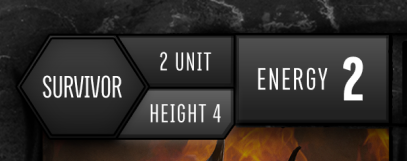
\includegraphics[width=0.8\linewidth]{chapters/charactercard/TimeStrikeCharCardTopLeft.png}
\end{figure}

\subsubsection{Bottom left:}
Name, Personality Trait, Race and Faction

\begin{figure}[ht]
    
\includegraphics[width=0.8\linewidth]{chapters/charactercard/TimeStrikeCharCardBottomLeft.png}
\end{figure}

\subsubsection{Top Middle:}
The Health Bar

\begin{figure}[ht]
    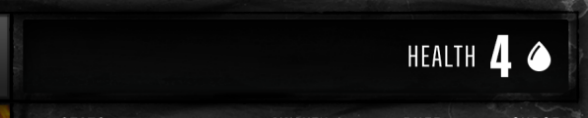
\includegraphics[width=0.8\linewidth]{chapters/charactercard/TimeStrikeCharCardHealth.png}
\end{figure}

\subsubsection{To the right of the character artwork shows:}
Stats, Movement Type, and Range Type
\begin{figure}[h]
    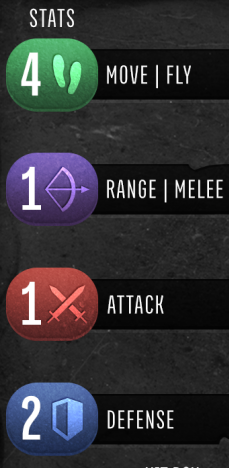
\includegraphics[width=0.3\linewidth]{chapters/charactercard/TimeStrikeCharCardStats.png}
\end{figure}

\subsubsection{Center:}
To the right of the stats are the status columns for Awaken, Buffs, and Curses. 
\tsgap
\begin{figure}[h]
    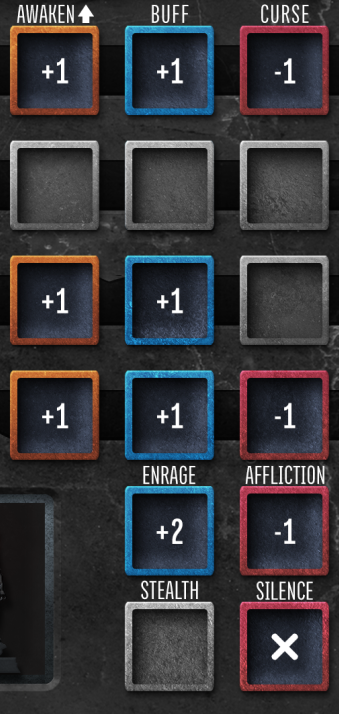
\includegraphics[width=0.8\linewidth]{chapters//charactercard/TimeStrikeCharCardStatusColumns.png}
\end{figure}

\subsubsection{Bottom Center:}
Below the stats is the hit box.   Parts that you can target and parts that you can not are visualized on the hit box. 
\tsgap

\begin{figure}[h]  
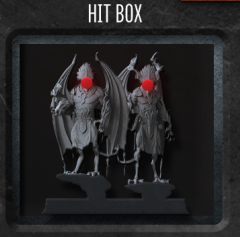
\includegraphics[width=0.75\linewidth]{chapters//charactercard/TimeStrikeCharCardHitbox.png}
\end{figure}

\subsubsection{Right:}
To the right of the cards is the skill sheet.
\begin{TimeStrikeTable}[]{XX}
    Top Left Text & The Skill Type.  \\
    Top Right Text & The Skill Name.  \\
    Lower Text  & How the Skill Works.
\end{TimeStrikeTable}

\begin{figure}[h]
\centering
    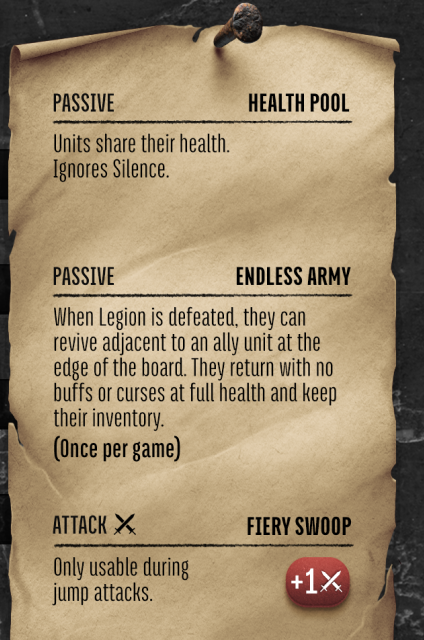
\includegraphics[width=0.75\linewidth]{chapters//charactercard/TimeStrikeCharCardSkills.png}
\end{figure}

\subsection{Back of Card}
    \normalsize The back of the Character card has some more information listed. It starts with the Character's name and a bit of their backstory. This is followed by their Role as well as a summary of their play style. 
  \tcbincludegraphics[blank]{chapters//charactercard/TimeStrikeCharCardback.png}
  
\clearpage

\end{document}
